% !TeX program = xelatex
\documentclass[12pt,a4paper]{article}

\usepackage{fontspec}
\setmainfont{Times New Roman}
\setsansfont{Arial}
\setmonofont{Consolas}

\usepackage[vietnamese]{babel}
\usepackage[a4paper,top=2.5cm,bottom=2.5cm,left=3cm,right=2.5cm]{geometry}
\usepackage{graphicx}
\usepackage{longtable}
\usepackage{booktabs}
\usepackage{array}
\usepackage[table]{xcolor}
\usepackage{hyperref}
\usepackage{titlesec}
\usepackage{fancyhdr}
\usepackage{caption}
\usepackage{enumitem}
\usepackage{float}
\usepackage{pifont}

\definecolor{headbg}{HTML}{EEF4FF}
\definecolor{rulecol}{HTML}{9DB8F2}
\definecolor{notebg}{HTML}{FFF9DB}
\definecolor{notestroke}{HTML}{E9D58A}

\hypersetup{colorlinks=true,linkcolor=blue!50!black,urlcolor=blue!60!black}
\setlength{\parskip}{5pt}
\setlength{\parindent}{0pt}
\captionsetup{font=small,labelsep=colon,justification=centering}
\setlist[itemize]{leftmargin=1.5em,itemsep=3pt,topsep=3pt}

\titleformat{\section}{\Large\bfseries\sffamily\color{black}}{\thesection.}{0.8em}{}
\titleformat{\subsection}{\large\bfseries\sffamily\color{black}}{\thesubsection}{0.6em}{}
\titlespacing*{\section}{0pt}{16pt}{6pt}
\titlespacing*{\subsection}{0pt}{11pt}{4pt}

\pagestyle{fancy}
\fancyhf{}
\setlength{\headheight}{14pt}
\lhead{\small\sffamily Báo cáo tiến độ GR2 --- Tuần 2}
\rhead{\small\sffamily Hoàng Kim Vĩnh --- 20235876}
\cfoot{\thepage}
\renewcommand{\headrulewidth}{0.4pt}

\begin{document}

\begin{titlepage}
\centering
\vspace*{2.2cm}
{\Huge\bfseries BÁO CÁO TIẾN ĐỘ TUẦN 2 (GR2)\par}
\vspace{0.5cm}
{\large Đề tài: thiết kế board điều khiển ổ cắm điện thông minh và tập trung\par}
\vspace{1.8cm}
\renewcommand{\arraystretch}{1.35}
\begin{tabular}{rl}
  \textbf{Sinh viên thực hiện:} & Hoàng Kim Vĩnh \\
  \textbf{MSSV:} & 20235876 \\
  \textbf{Lớp:} & Việt Nhật 01 \\
  \textbf{Trường:} & Đại học Bách khoa Hà Nội \\
  \textbf{GVHD:} & Nguyễn Đức Tiến \\
  \textbf{Ngày:} & 17 tháng 11 năm 2026 \\
\end{tabular}
\vfill
{\small Báo cáo tiến độ GR2 --- Tuần 2 --- Hoàng Kim Vĩnh --- 20235876\par}
\end{titlepage}
\tableofcontents
\newpage
\section{Tổng quan tiến độ}
Tiếp nối kết quả của Tuần 1 (xây dựng thành công ứng dụng web đọc thông số điện năng từ module PZEM-004T V3.0 qua cổng nối tiếp), tại buổi báo cáo trước, Giảng viên hướng dẫn đã chỉ ra rằng hệ thống cần vượt qua giới hạn của một công cụ thử nghiệm chạy tay để trở thành một thành phần mang tính sản phẩm thực tế trong tủ rack máy chủ.

Trong Tuần 2, em đã tập trung giải quyết trọn vẹn 10 yêu cầu từ Giảng viên thông qua hai trọng tâm chính:

\begin{itemize}
  \item \textbf{Chuyển đổi sang dịch vụ nền 24/7 (Electronic PC Agent):} Tái cấu trúc mã nguồn thành một dịch vụ nền chạy tự động trên Windows, tích hợp cơ chế tự dò cổng giao tiếp, lưu trữ dữ liệu lịch sử, cảnh báo sự cố độc lập và tăng cường bảo mật vận hành.
  \item \textbf{Đóng gói và phát hành thư viện dùng chung:} Tách các thành phần giao thức và xử lý lõi thành thư viện C99 chuẩn mang tên embedded-iot-toolkit và đăng ký thành công lên cả hai kho lưu trữ công khai là Arduino Library Manager và ESP-IDF Component Registry.
\end{itemize}
Hiện tại, toàn bộ phần mềm của Giai đoạn 1 (12/12 hạng mục ưu tiên) đã hoàn thiện và vượt qua 36 kịch bản kiểm thử tự động. Các hạng mục kiểm thử thực tế phụ thuộc vào phần cứng và môi trường máy chủ vật lý được phân tách rõ ràng sang Giai đoạn 2.

\section{Những nội dung đã tìm hiểu về dịch vụ nền trên Windows}
Song song với phần hiện thực, em đã dành thời gian tìm hiểu sâu về cách vận hành một dịch vụ nền (service) trên Windows, bởi đây là điểm mới hoàn toàn so với mô hình script chạy tay của Tuần 1. Dưới đây là tóm tắt các nội dung đã tìm hiểu và ứng dụng thực tế của chúng.

\noindent\textbf{Service Control Manager (SCM) và vòng đời một Windows Service.} Em đã học được rằng một service không đơn thuần là một chương trình chạy nền, mà phải đi qua một vòng đời do SCM điều phối: đăng ký service, SCM gọi lệnh khởi động, tiến trình phải báo trạng thái RUNNING, và khi dừng thì phải trả lời lệnh dừng trước khi thoát. Chính vì vậy trong mã nguồn, phần khởi tạo được tách thành các hàm rõ ràng (Initialize, PrepareToHostSingle, StartServiceCtrlDispatcher, SvcDoRun, SvcStop) thay vì một vòng lặp vô tận, để SCM có thể điều khiển vòng đời một cách đúng đắn.\par
\noindent\textbf{Cơ chế tự phục hồi (Crash Recovery) của SCM và cấu hình FailureActions.} Em tìm hiểu rằng SCM cho phép cấu hình hành động khi service chết, ví dụ khởi động lại sau 5 giây, sau 10 giây và sau 30 giây, kèm bộ đếm reset trong 24 giờ. Nhờ đó một sự cố tạm thời (tiến trình bị kill, rớt kết nối USB-TTL) không khiến hệ thống phải can thiệp thủ công. Bộ cấu hình này đã được đưa vào script cài đặt cùng với cơ chế tự khởi động trễ.\par
\noindent\textbf{Session 0 và những điều service không được phép làm.} Đây là điểm em tìm hiểu kỹ nhất và cũng là bẫy thực tế. Service chạy trong Session 0 tách biệt hoàn toàn khỏi phiên đăng nhập của người dùng, nên nó không có console, và trong Python các biến sys.stdout và sys.stderr có thể bằng None, khiến một lệnh in đơn giản ném ra lỗi AttributeError làm sập cả tiến trình. Vì vậy phần ghi log được thiết kế để luôn ghi ra file với cơ chế xoay vòng (10 MB × 10 bản), và chỉ gắn thêm handler ghi ra console khi kiểm tra được stdout thực sự dùng được.\par
\noindent\textbf{Sự khác biệt giữa các lớp đăng ký service và vì sao chọn pywin32.} Em đã so sánh nhiều phương án: dùng ServiceFramework của pywin32, dùng wrapper có sẵn pythonservice.exe của pywin32, hay dùng wrapper ngoài như NSSM và WinSW. Điểm quan trọng em tìm hiểu được là wrapper pythonservice.exe bị liên kết cứng với thư viện DLL của bản Python gốc và không đọc tệp pyvenv.cfg, nên service sẽ chạy bằng Python gốc, mất đi thư viện pyserial đã cài trong môi trường ảo. Cách khắc phục là trỏ ImagePath thẳng vào python.exe của môi trường ảo để python.exe làm host trực tiếp. Đối với NSSM và WinSW, em loại vì cần binary ngoài và NSSM đã ngừng phát hành từ năm 2014, thường bị phần mềm bảo mật coi là công cụ đáng ngờ.\par
\noindent\textbf{Cơ chế tự khởi động và quyền truy cập cổng COM của tài khoản dịch vụ.} Em đã tìm hiểu cơ chế tự khởi động trễ (delayed auto-start) nhằm tránh tranh chấp I/O với các dịch vụ khác trong lúc máy khởi động, đồng thời tìm hiểu về quyền đọc cổng COM khi tiến trình chạy dưới tài khoản LocalSystem trong Session 0. Đây là điểm em ghi nhận là chưa kiểm chứng được bằng thực tế, nên đã đưa vào danh sách công việc của Giai đoạn 2.\par
\noindent\textbf{Ghi cấu hình nguyên tử (atomic write) để tránh mất cấu hình khi máy mất điện.} Em tìm hiểu rằng nếu ghi thẳng vào tệp cấu hình và bị mất điện giữa chừng, tệp có thể bị hỏng hoặc chứa dữ liệu dở dang, khiến service không khởi động được. Cách an toàn là ghi ra một tệp tạm trong cùng thư mục, flush xuống đĩa, gọi fsync để bắt buộc hệ điều hành ghi thật, rồi dùng os.replace để thay thế tệp đích một cách nguyên tử. Kỹ thuật này được áp dụng cho tệp cấu hình nơi lưu cổng COM đã dò được.\par
\noindent\textbf{Cơ chế xoay vòng tệp log để chống tràn đĩa khi chạy dài ngày.} Một service chạy 24/7 sẽ sinh log liên tục nếu không kiểm soát. Em đã tìm hiểu và áp dụng RotatingFileHandler của Python với giới hạn 10 MB mỗi bản và giữ lại 10 bản, nhờ đó dung lượng log luôn được kiểm soát mà không cần can thiệp thủ công xoá.\par
\noindent\textbf{Tích hợp cơ sở dữ liệu SQLite ở chế độ WAL cho bài toán ghi và đọc đồng thời.} Do vòng lấy mẫu chạy liên tục 1 Hz trong khi giao diện web vẫn cần truy vấn dữ liệu, em đã tìm hiểu cơ chế WAL (Write-Ahead Logging) của SQLite. Ở chế độ này, một tiến trình đọc không bị chặn bởi tiến trình đang ghi, khác với chế độ mặc định. Kết hợp với synchronous=NORMAL, toàn bộ lịch sử đo được ghi liên tục mà giao diện vẫn truy vấn mượt mà.\par
\section{Những gì đã làm trong Giai đoạn 1}
Trong Giai đoạn 1, toàn bộ công việc của Tuần 2 được tổ chức thành 12 hạng mục ưu tiên và đều đã hoàn thành. Dưới đây là tổng hợp những gì đã thực hiện, theo thứ tự các nhóm công việc.

Trước hết, toàn bộ mã nguồn cũ đã được tái cấu trúc thành một package độc lập có tên pc\textbackslash{}\_agent, với ranh giới rõ rệt giữa bốn tầng: tầng driver (đọc thiết bị), tầng lõi xử lý (vòng lấy mẫu và bộ luật), tầng lưu trữ (cơ sở dữ liệu) và tầng giao diện (REST API cùng dashboard). Song song, mô hình dữ liệu được thiết kế theo phân cấp Site → Rack → Meter và áp dụng xuyên suốt từ tầng cấu hình cho tới cơ sở dữ liệu, để phù hợp với bài toán giám sát một tổ hợp máy chủ trong tủ rack.

Tiếp theo, ứng dụng web chạy tay của Tuần 1 đã được chuyển thành một dịch vụ nền chạy dưới dạng Windows Service (SCM) trên nền tảng Windows, với cấu hình tự khởi động cùng hệ điều hành và cơ chế tự khởi động lại theo chu kỳ khi gặp sự cố. Dịch vụ hoàn toàn không có giao diện đồ họa, chạy trong Session 0 và không cần đăng nhập người dùng.

Để giải quyết triệt để vấn đề cổng COM đổi số mỗi khi cắm lại cáp USB-TTL, đã xây dựng thuật toán dò tìm 4 bậc với điều kiện xác minh nghiêm ngặt (đúng function code, đúng byte count, CRC-16 hợp lệ, dải điện áp và tần số nằm trong ngưỡng lưới điện thực tế). Cổng đã dò được được lưu lại bằng cơ chế ghi cấu hình nguyên tử kèm chống ghi đè giá trị lỗi, nên sau lần cắm lại cáp, dịch vụ vẫn tìm được đúng thiết bị mà không cần thao tác tay.

Phần lưu trữ dữ liệu chuỗi thời gian cũng đã được bổ sung: toàn bộ số đo được ghi xuống cơ sở dữ liệu SQLite ở chế độ WAL, với mẫu thô giữ trong 14 ngày phục vụ chẩn đoán chi tiết và số liệu tổng hợp theo giờ (min/max/trung bình, hệ số tải) giữ trong 365 ngày để theo dõi dài hạn, kèm cơ chế tự động dọn dẹp và sao lưu định kỳ hằng ngày. Chế độ WAL cho phép giao diện truy vấn dữ liệu mượt mà ngay cả khi dịch vụ nền vẫn đang ghi mẫu liên tục ở chu kỳ 1 Hz.

Bên cạnh đó, một bộ luật giám sát (Rule Engine) đã được tích hợp để nhận diện 6 loại sự cố điện năng gồm quá công suất, quá dòng, quá áp, sụt áp, báo động nội tại của module và mất kết nối thiết bị. Bộ luật chạy ngay trong tiến trình của dịch vụ với độ trễ dưới 1 ms, nhờ đó hệ thống vẫn phát hiện sự cố và gửi thông báo ngay cả khi mất kết nối tới máy chủ trung tâm. Các cảnh báo được tự động đóng khi tình trạng trở lại an toàn, tránh gửi thông báo lặp. Dashboard tích hợp sẵn được thiết kế không phụ thuộc thư viện ngoài (không dùng CDN) và yêu cầu xác thực Bearer Token khi mở truy cập ra mạng LAN.

Mô hình kiến trúc tổng quát cũng đã được làm rõ: toàn bộ hệ thống được phân tách thành ba thành phần độc lập (PC Agent ở tầng biên, Web Server ở tầng trình diễn và Vi điều khiển ESP32-S3 ở tầng chấp hành), kèm tài liệu kiến trúc và các sơ đồ mô tả luồng dữ liệu. Đồng thời, hạ tầng vật lý (Serial) và tầng giao thức (Modbus) được tách biệt hoàn toàn, nhờ đó phần truyền dẫn cổng nối tiếp và phần đóng/giải mã khung dữ liệu Modbus-RTU có thể kiểm thử độc lập, và chỉ cần thay thiết bị Modbus khác là toàn bộ tầng trên vẫn giữ nguyên.

Các khối mã lặp lại giữa tầng PC và tầng vi điều khiển (bộ định thời không chặn, đóng khung dữ liệu nối tiếp có kiểm tra lỗi, phát hiện dữ liệu cảm biến bị treo) đã được tách thành một thư viện C99 thuần túy dùng chung, mang tên embedded-iot-toolkit, và đã được phát hành công khai trên cả Arduino Library Manager lẫn ESP-IDF Component Registry (chi tiết ở mục 4.3).

Cuối cùng, phần tài liệu vận hành đã được hoàn thiện gồm hướng dẫn cài đặt từ đầu, danh mục lỗi thường gặp và hướng dẫn chuẩn bị phần cứng cho Giai đoạn 2; đồng thời đã xây dựng bộ kiểm thử tự động gồm 36 kịch bản bao phủ giải mã khung truyền, xác thực token, lưu trữ và kích hoạt cảnh báo, tất cả đều đạt.

\section{Kết quả thiết kế và hiện thực hệ thống}
\subsection{Kiến trúc tổng thể 3 thành phần}
Để khắc phục tình trạng xung đột truy cập cổng COM (vốn chỉ cho phép một tiến trình chiếm giữ tại một thời điểm trên Windows) và đảm bảo tính sẵn sàng cao trong tủ rack, hệ thống được phân tách thành ba thành phần độc lập:

\begin{itemize}
  \item \textbf{Electronic PC Agent (Tầng biên):} Chạy ngầm trực tiếp trên máy chủ giám sát, giữ độc quyền kết nối USB-TTL với PZEM-004T, thu thập dữ liệu, lưu trữ cục bộ và xử lý cảnh báo tại chỗ.
  \item \textbf{Web Server (Tầng trình diễn):} Giao tiếp với PC Agent qua REST API/MQTT để cung cấp giao diện quản trị tập trung cho nhiều tủ rack mà không can thiệp trực tiếp vào phần cứng nối tiếp.
  \item \textbf{Central IoT Controller – ESP32-S3 (Tầng chấp hành):} Đảm nhiệm việc đóng cắt relay cách ly nguồn điện khi có lệnh điều khiển hoặc tình huống khẩn cấp.
\end{itemize}
\begin{figure}[H]
\centering
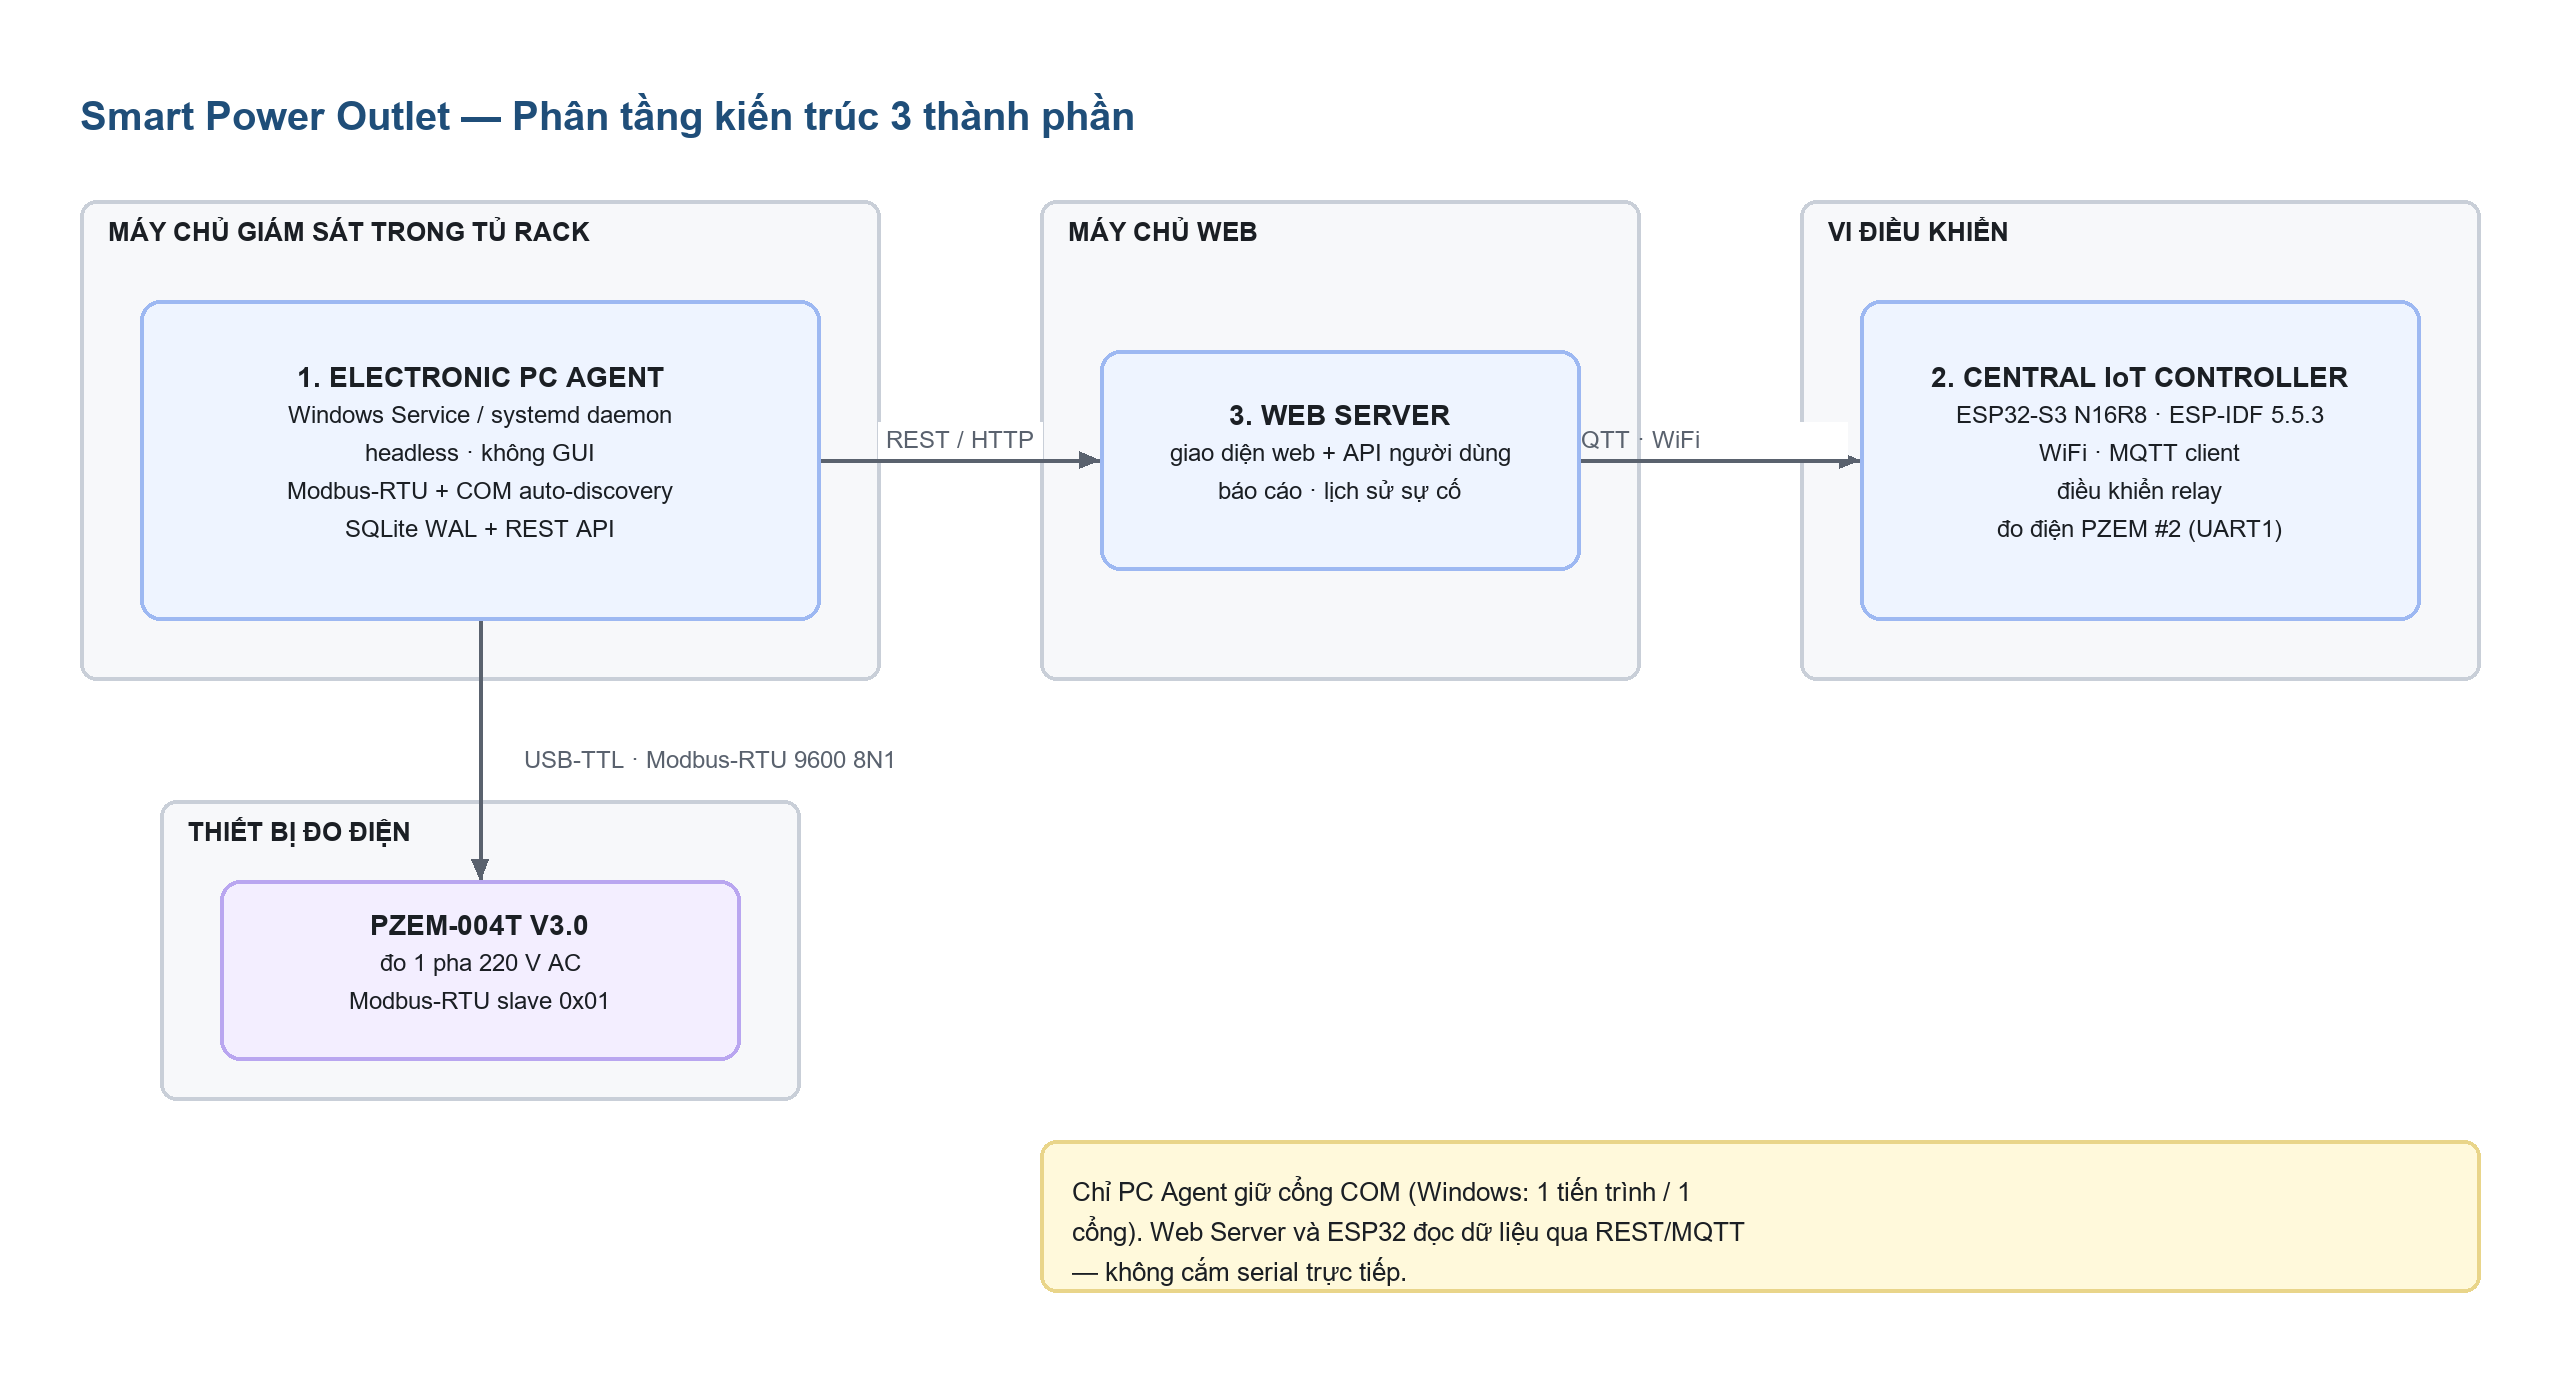
\includegraphics[width=\linewidth]{architecture_tiers.png}
\caption{Mô hình phân tầng kiến trúc 3 thành phần của hệ thống giám sát năng lượng}
\label{fig:architecture}
\end{figure}
\subsection{Các tính năng cốt lõi của Electronic PC Agent}
\noindent\textbf{1. Tự động dò tìm và phục hồi kết nối (COM Auto-Discovery):} Thay vì cố định tên cổng COM vốn dễ thay đổi mỗi khi cắm lại cáp USB-TTL trên Windows, hệ thống áp dụng chiến lược dò tìm 4 bậc ưu tiên: thử lại cổng đã lưu trong bộ nhớ đệm → đối chiếu vị trí vật lý cổng USB (USB topology) → lọc danh sách cổng theo mã định danh chip chuyển đổi (CH340, CP210x, FTDI) → quét toàn dải địa chỉ. Một cổng chỉ được công nhận khi phản hồi đúng cấu trúc Modbus, hợp lệ mã CRC-16 và trả về dải điện áp, tần số nằm trong ngưỡng lưới điện thực tế.\par
\noindent\textbf{2. Lưu trữ dữ liệu chuỗi thời gian (Time-Series Storage):} Hệ thống sử dụng cơ sở dữ liệu SQLite kích hoạt chế độ ghi đồng thời (WAL), cho phép giao diện web truy vấn dữ liệu mượt mà trong lúc dịch vụ nền vẫn đang ghi mẫu liên tục. Dữ liệu được phân tầng lưu trữ: mẫu đo thô lưu trong 14 ngày phục vụ chẩn đoán chi tiết, và dữ liệu tổng hợp theo giờ (min/max/trung bình, hệ số tải) lưu trong 365 ngày để theo dõi dài hạn, kèm cơ chế tự động dọn dẹp và sao lưu định kỳ mỗi ngày.\par
\noindent\textbf{3. Giám sát sự cố tại chỗ và bảo mật vận hành:} Bộ đánh giá ngưỡng (Rule Engine) hoạt động trực tiếp trong tiến trình của Agent với độ trễ dưới 1 ms, nhận diện 6 trạng thái bất thường: quá công suất, quá dòng, quá áp, sụt áp (theo tiêu chuẩn dải áp 198–242 V của tủ rack), báo động nội tại của module và mất kết nối thiết bị. Việc xử lý tại chỗ đảm bảo hệ thống vẫn phát hiện sự cố và gửi thông báo qua Telegram ngay cả khi mất kết nối tới máy chủ trung tâm. Ngoài ra, giao diện dashboard tích hợp sẵn được thiết kế không phụ thuộc thư viện ngoài (không dùng CDN) và yêu cầu xác thực Bearer Token khi mở truy cập ra mạng LAN.\par
\subsection{Phát hành thư viện dùng chung embedded-iot-toolkit}
Trong quá trình phát triển từ GR1 sang GR2, nhiều bài toán kỹ thuật như bộ định thời không chặn (thay thế delay()), đóng khung dữ liệu nối tiếp có kiểm tra lỗi và phát hiện dữ liệu cảm biến bị treo (stale data) phải viết lặp lại ở cả tầng PC (Python) và vi điều khiển (C/C++). Trong tuần qua, em đã tách các khối chức năng này thành thư viện chuẩn C99 thuần túy (embedded-iot-toolkit), không phụ thuộc phần cứng cụ thể, và phát hành chính thức phiên bản 1.0.0 lên cả hai hệ sinh thái phổ biến nhất:

\begin{itemize}
  \item \textbf{Arduino Library Manager:} Đã vượt qua kiểm duyệt tiêu chuẩn nghiêm ngặt và được hợp nhất vào kho chính thức (PR \textbackslash{}\#9655).
  \item \textbf{ESP-IDF Component Registry:} Đã xuất bản tại địa chỉ catkod/embedded-iot-toolkit và kiểm chứng thực tế bằng cách khởi tạo một dự án ESP32-S3 mới, tải thư viện trực tiếp từ registry và biên dịch thành công.
\end{itemize}
\begin{figure}[H]
\centering
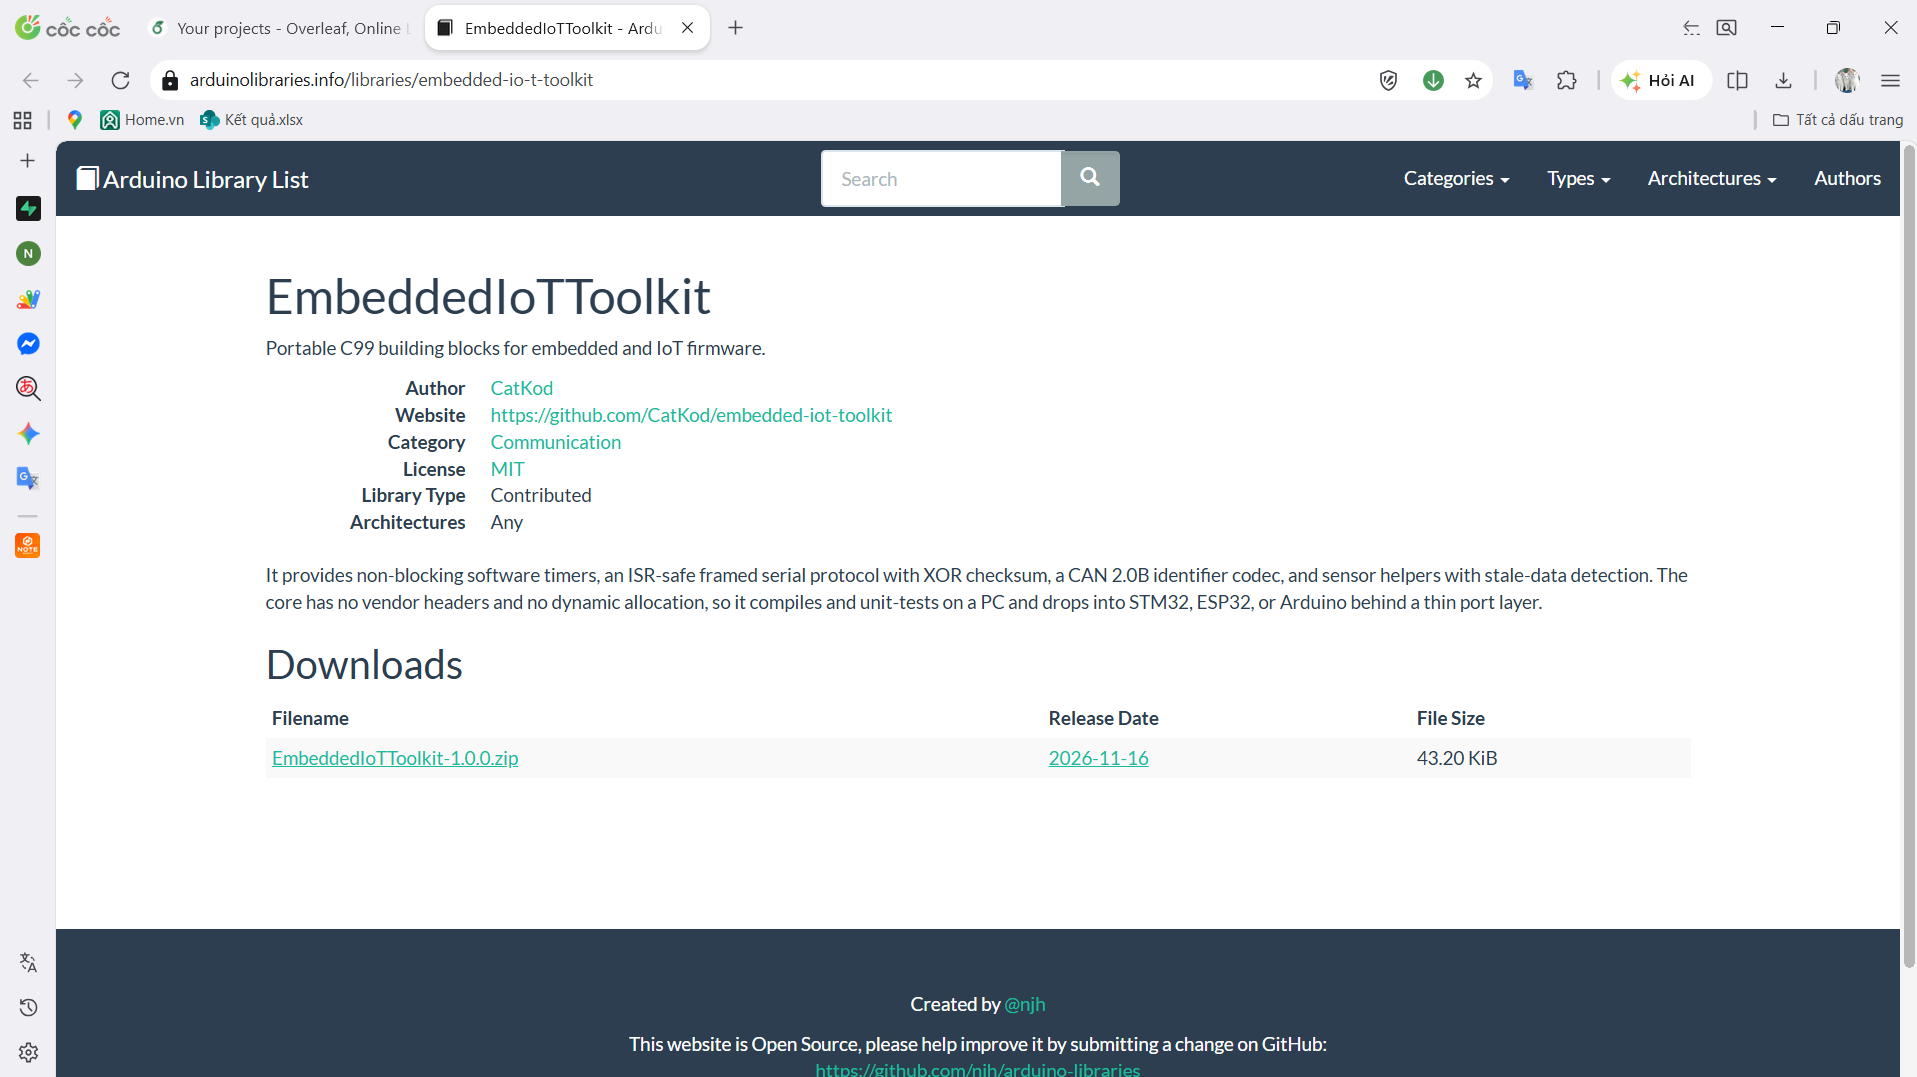
\includegraphics[width=0.82\linewidth]{Arduino.png}
\caption{Minh chứng phát hành thư viện embedded-iot-toolkit v1.0.0 trên Arduino Library Manager}
\label{fig:arduino}
\end{figure}
\begin{figure}[H]
\centering
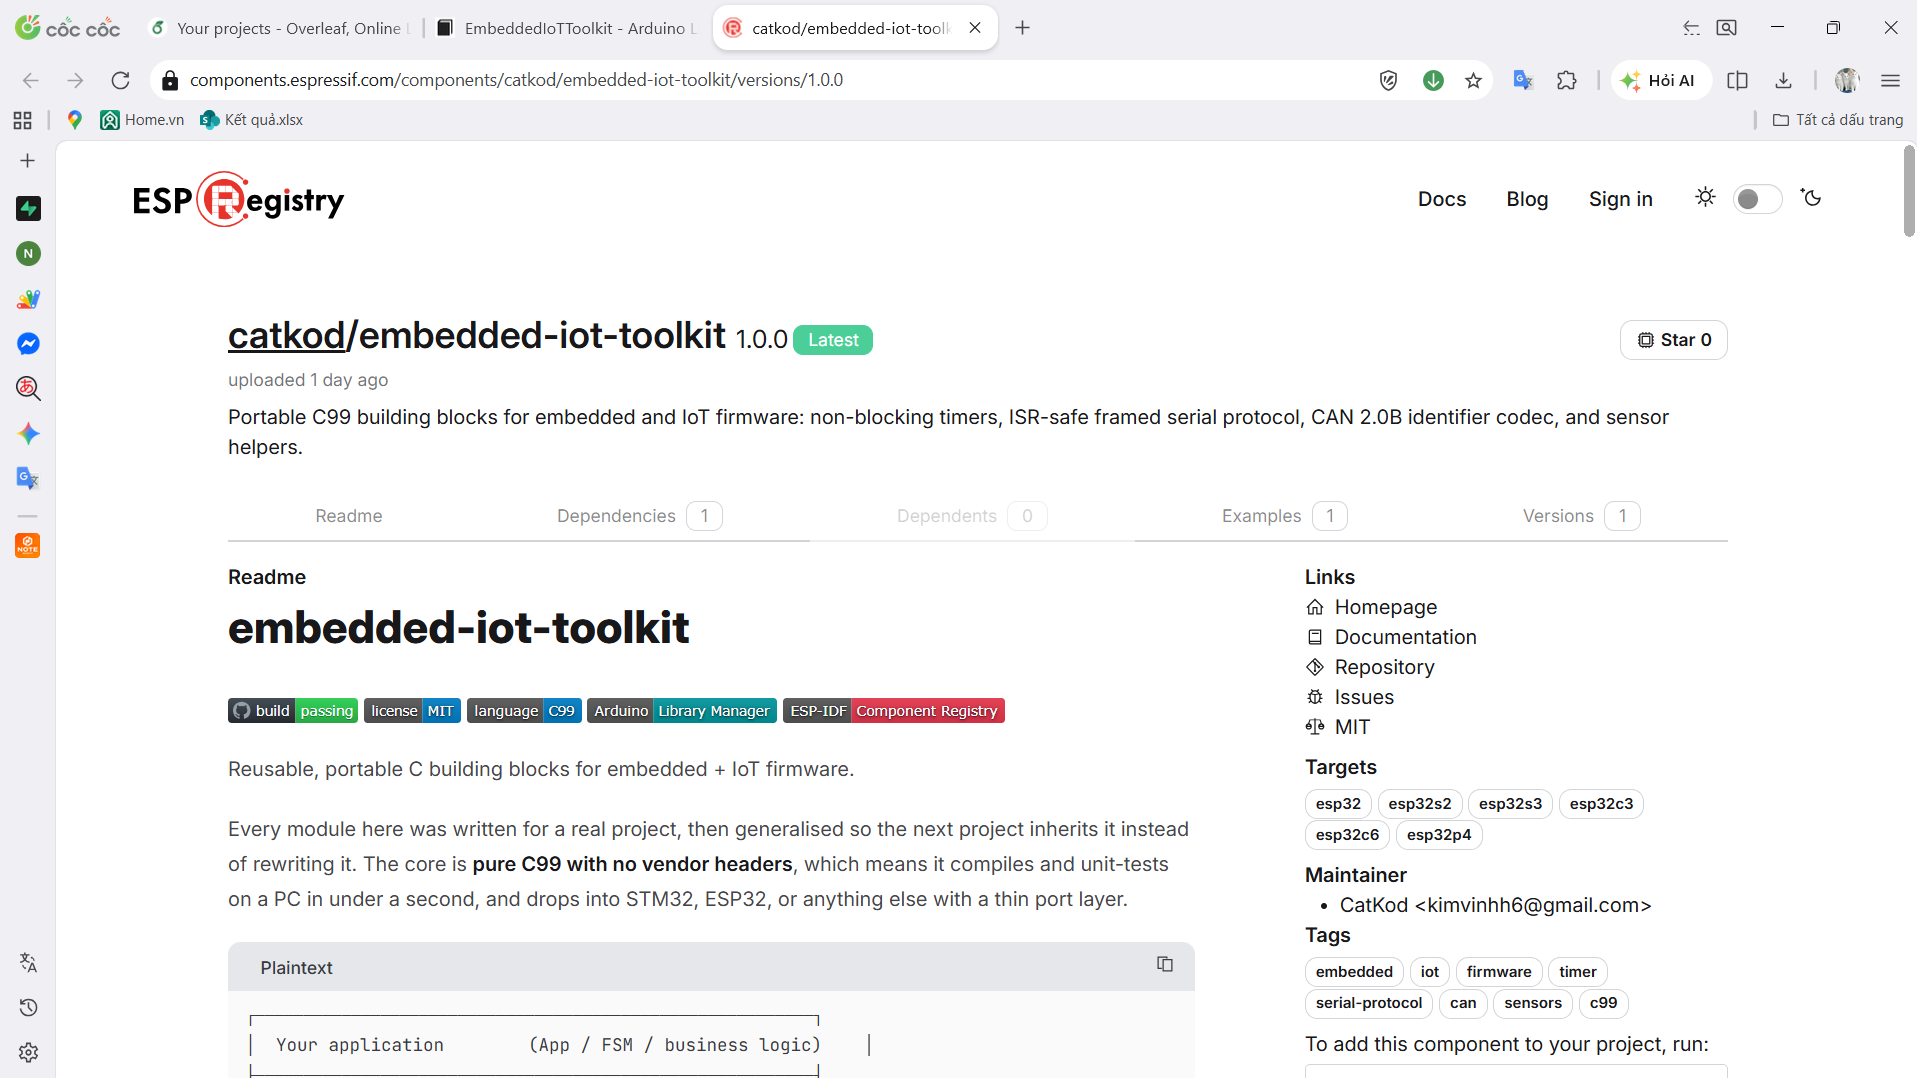
\includegraphics[width=0.82\linewidth]{Esp-idf.png}
\caption{Minh chứng phát hành thư viện embedded-iot-toolkit v1.0.0 trên ESP-IDF Component Registry (catkod/embedded-iot-toolkit)}
\label{fig:espidf}
\end{figure}
\section{Kiểm thử và khắc phục sự cố phát sinh}
Hệ thống đã được kiểm chứng qua bộ 36 kịch bản kiểm thử tự động (đạt tỷ lệ 100\%) bao phủ toàn bộ các chức năng giải mã khung truyền, bảo mật token, lưu trữ và kích hoạt cảnh báo. Đặc biệt, thông qua công cụ chạy thử nghiệm liên tục (soak test), em đã chủ động phát hiện và khắc phục triệt để 2 lỗi nghiêm trọng có nguy cơ gây treo hệ thống khi vận hành dài ngày:

\noindent\textbf{1. Lỗi khóa cơ sở dữ liệu (Database table is locked):} Do quản lý phiên kết nối SQLite chưa giải phóng tài nguyên đúng cách sau mỗi chu kỳ ghi, gây rò rỉ handle. Đã khắc phục bằng cách bọc cơ chế tự động đóng kết nối sau mỗi giao dịch.\par
\noindent\textbf{2. Lỗi không dọn dẹp dữ liệu cũ:} Do sai sót cú pháp tham số truy vấn khiến tiến trình xóa dữ liệu quá hạn không thực thi và xung đột lệnh kiểm tra bộ nhớ đệm WAL. Đã chuẩn hóa lại cấu trúc truy vấn và tách biệt tiến trình bảo trì.\par
\end{document}